%\section*{\begin{center}{\Huge Appendix}\end{center}}
\addcontentsline{toc}{chapter}{Appendix}
\chapter{Plots}\label{Appendix}

\begin{figure}[H]
    \centering
    \subfloat[DQN]{
        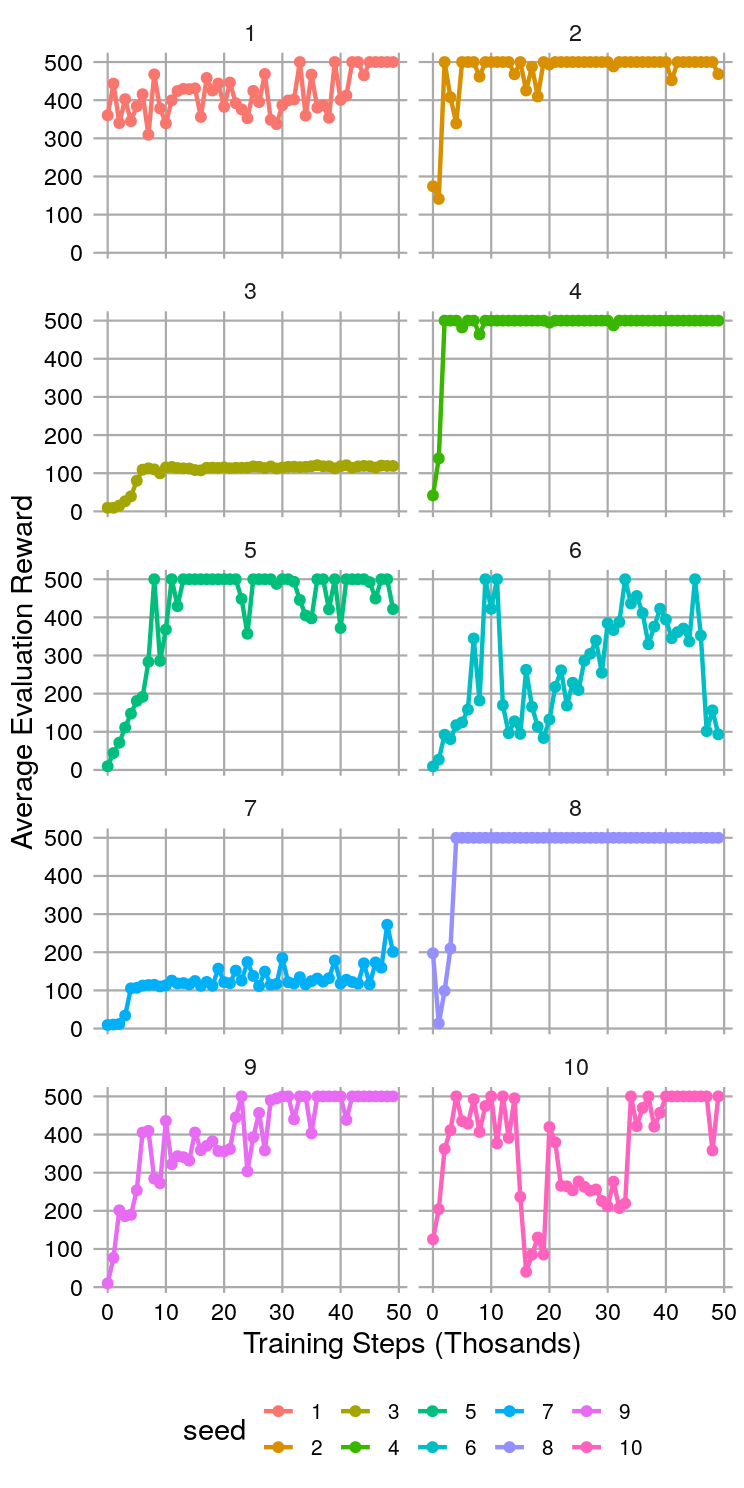
\includegraphics[scale=0.5]{PerDQNCartpole.png}
    }
    \subfloat[BNIG DQN]{
        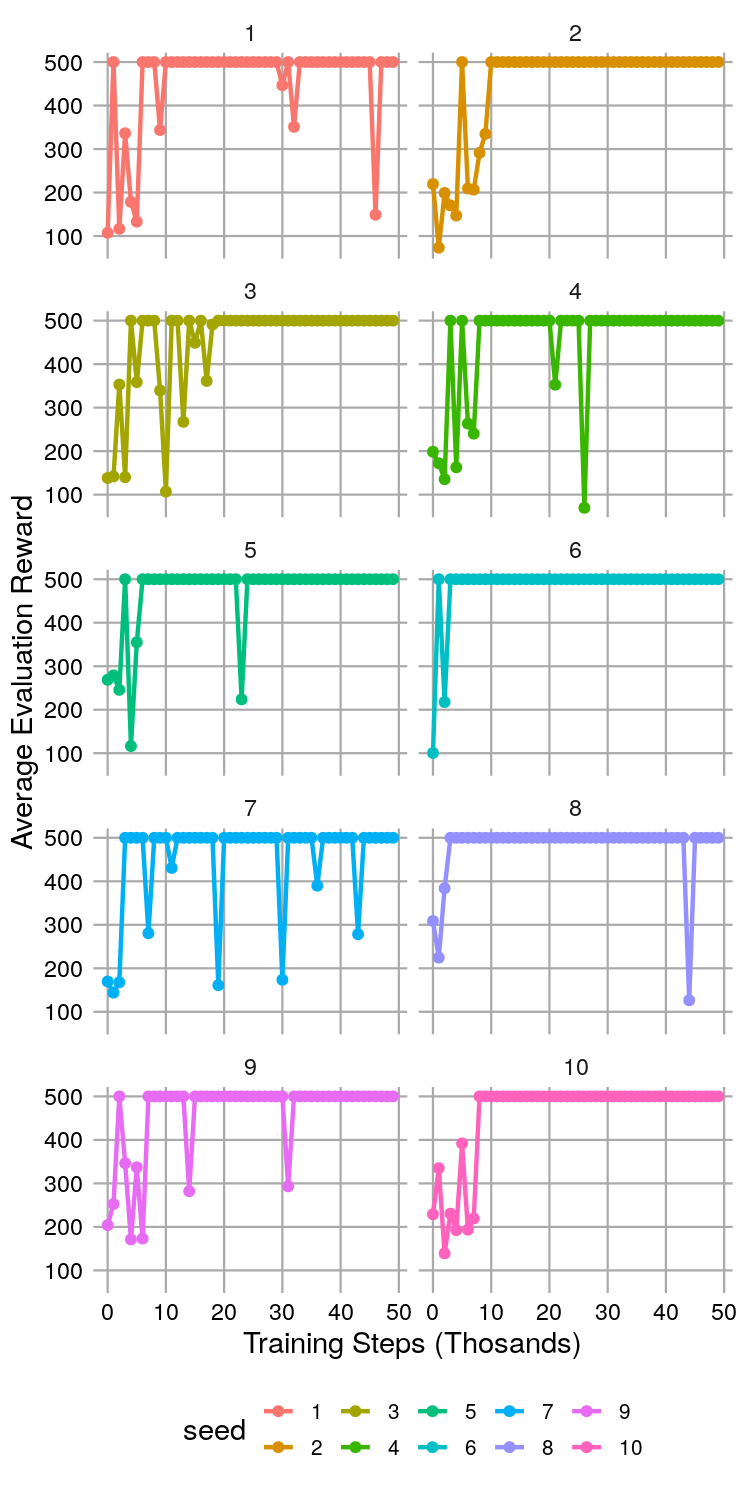
\includegraphics[scale=0.5]{PerBDQNCartpole.png}
    }
    \caption{\textbf{Per Seed DQN and BNIG DQN Performance on Cartpole}: Each color represents a new attempt. Note the unstable performance of DQN when it has found a good policy and that some attempts it never finds an optimal policy.}
    \label{fig:nn_per_cartpole}
\end{figure}
